% Why do we need to submit this? It's not part of the markscheme and you wouldn't
% usually give out your TeX code, just the PDF.

% -------------------------------------------------------------------------------
% Establish page structure & font.
\documentclass[12pt]{report}\usepackage[]{graphicx}\usepackage[]{xcolor}
% maxwidth is the original width if it is less than linewidth
% otherwise use linewidth (to make sure the graphics do not exceed the margin)
\makeatletter
\def\maxwidth{ %
  \ifdim\Gin@nat@width>\linewidth
    \linewidth
  \else
    \Gin@nat@width
  \fi
}
\makeatother

\definecolor{fgcolor}{rgb}{0.345, 0.345, 0.345}
\newcommand{\hlnum}[1]{\textcolor[rgb]{0.686,0.059,0.569}{#1}}%
\newcommand{\hlstr}[1]{\textcolor[rgb]{0.192,0.494,0.8}{#1}}%
\newcommand{\hlcom}[1]{\textcolor[rgb]{0.678,0.584,0.686}{\textit{#1}}}%
\newcommand{\hlopt}[1]{\textcolor[rgb]{0,0,0}{#1}}%
\newcommand{\hlstd}[1]{\textcolor[rgb]{0.345,0.345,0.345}{#1}}%
\newcommand{\hlkwa}[1]{\textcolor[rgb]{0.161,0.373,0.58}{\textbf{#1}}}%
\newcommand{\hlkwb}[1]{\textcolor[rgb]{0.69,0.353,0.396}{#1}}%
\newcommand{\hlkwc}[1]{\textcolor[rgb]{0.333,0.667,0.333}{#1}}%
\newcommand{\hlkwd}[1]{\textcolor[rgb]{0.737,0.353,0.396}{\textbf{#1}}}%
\let\hlipl\hlkwb

\usepackage{framed}
\makeatletter
\newenvironment{kframe}{%
 \def\at@end@of@kframe{}%
 \ifinner\ifhmode%
  \def\at@end@of@kframe{\end{minipage}}%
  \begin{minipage}{\columnwidth}%
 \fi\fi%
 \def\FrameCommand##1{\hskip\@totalleftmargin \hskip-\fboxsep
 \colorbox{shadecolor}{##1}\hskip-\fboxsep
     % There is no \\@totalrightmargin, so:
     \hskip-\linewidth \hskip-\@totalleftmargin \hskip\columnwidth}%
 \MakeFramed {\advance\hsize-\width
   \@totalleftmargin\z@ \linewidth\hsize
   \@setminipage}}%
 {\par\unskip\endMakeFramed%
 \at@end@of@kframe}
\makeatother

\definecolor{shadecolor}{rgb}{.97, .97, .97}
\definecolor{messagecolor}{rgb}{0, 0, 0}
\definecolor{warningcolor}{rgb}{1, 0, 1}
\definecolor{errorcolor}{rgb}{1, 0, 0}
\newenvironment{knitrout}{}{} % an empty environment to be redefined in TeX

\usepackage{alltt}

\usepackage[total={6.5in, 9in},
	left=1in,
	right=1in,
	top=1in,
	bottom=1in,]{geometry} % Page structure

\usepackage{graphicx} % Required for inserting images
\graphicspath{{images/}} % Any additional images I use (BCU logo, etc) are from here.

\usepackage[utf8]{inputenc} % UTF-8 encoding
\usepackage[T1]{fontenc} % T1 font
\usepackage{float}  % Allows for floats to be positioned using [H], which correctly
                    % positions them relative to their location within my LaTeX code.
\usepackage{subcaption}

% -------------------------------------------------------------------------------
% Declare biblatex with custom Harvard BCU styling for referencing.
\usepackage[
    useprefix=true,
    maxcitenames=3,
    maxbibnames=99,
    style=authoryear,
    dashed=false, 
    natbib=true,
    url=false
]{biblatex}

% Additional styling options to ensure Harvard referencing format.
\renewbibmacro*{volume+number+eid}{
    \printfield{volume}
    \setunit*{\addnbspace}
    \printfield{number}
    \setunit{\addcomma\space}
    \printfield{eid}}
\DeclareFieldFormat[article]{number}{\mkbibparens{#1}}

% Declare it as the bibliography source, to be called later via \printbibliography
\addbibresource{report.bib}

% -------------------------------------------------------------------------------
% To prevent "Chapter N" display for each chapter
\usepackage[compact]{titlesec}
\usepackage{wasysym}
\usepackage{import}

\titlespacing*{\chapter}{0pt}{-2cm}{0.5cm}
\titleformat{\chapter}[display]
{\normalfont\bfseries}{}{0pt}{\Huge}

% -------------------------------------------------------------------------------
% Custom macro to make an un-numbered footnote.

\newcommand\blfootnote[1]{
    \begingroup
    \renewcommand\thefootnote{}\footnote{#1}
    \addtocounter{footnote}{-1}
    \endgroup
}

% -------------------------------------------------------------------------------
% Fancy headers; used to show my name, BCU logo and current chapter for the page.
\usepackage{fancyhdr}
\usepackage{calc}
\pagestyle{fancy}

\setlength\headheight{37pt} % Set custom header height to fit the image.

\renewcommand{\chaptermark}[1]{%
    \markboth{#1}{}} % Include chapter name.


% Lewis Higgins - ID 22133848           [BCU LOGO]                [CHAPTER NAME]
\lhead{Lewis Higgins - ID 22133848~~~~~~~~~~~~~~~
\includegraphics[width=1.75cm]{bcu logo}}
\fancyhead[R]{\leftmark}


% Temp for pagecolor command
\usepackage{xcolor}

% -------------------------------------------------------------------------------

\title{CMP5352 Report - TITLE NEEDED}
\author{Lewis Higgins - Student ID 22133848}
\date{April 2024}

% -------------------------------------------------------------------------------
\IfFileExists{upquote.sty}{\usepackage{upquote}}{}
\begin{document}






 \pagecolor{yellow} % Change in final



    \makeatletter
    \begin{titlepage}
        \begin{center}
            
\includegraphics[width=0.7\linewidth]{bcu logo}\\[4ex]
            {\large \bfseries  \@title }\\[2ex]
            {\large \bfseries  DRAFT VERSION }\\[2ex]
            {\@author}\\[30ex]
            {Word count: XXXX}\\[20ex]
        \end{center}
    \end{titlepage}
    \makeatother
    \thispagestyle{empty}
    \newpage

  \pagecolor{white} % Change in final

    \begin{abstract}
        text

        text

        text

    \end{abstract} 
    
    % Page counter trick so that the contents page doesn't increment it.
    \setcounter{page}{0}

    \tableofcontents
    \thispagestyle{empty}

    % Declaring un-numbered chapter because I prefer how it looks.
    \chapter*{Introduction}\label{ch:introduction}
    % Add it to the contents, because un-numbered chapters aren't by default.
    \addcontentsline{toc}{chapter}{Introduction}
    % Put the chapter name in the header.
    \markboth{Introduction}{}

    Text text text

    Text text text

    \pagebreak

    % Declaring un-numbered chapter because I prefer how it looks.
    \chapter*{Motivation and objectives}\label{ch:sec1}
    % Add it to the contents, because un-numbered chapters aren't by default.
    \addcontentsline{toc}{chapter}{Motivation and objectives}
    % Put the chapter name in the header.
    \markboth{Motivation and objectives}{}

\begin{knitrout}
\definecolor{shadecolor}{rgb}{0.969, 0.969, 0.969}\color{fgcolor}\begin{kframe}
\begin{alltt}
\hlkwd{ggplot}\hlstd{(diamonds,} \hlkwd{aes}\hlstd{(}\hlkwc{x} \hlstd{= carat,} \hlkwc{fill} \hlstd{= color))} \hlopt{+}
  \hlkwd{geom_histogram}\hlstd{(}\hlkwc{bins} \hlstd{=} \hlnum{30}\hlstd{)}
\end{alltt}
\end{kframe}\begin{figure}[H]

{\centering 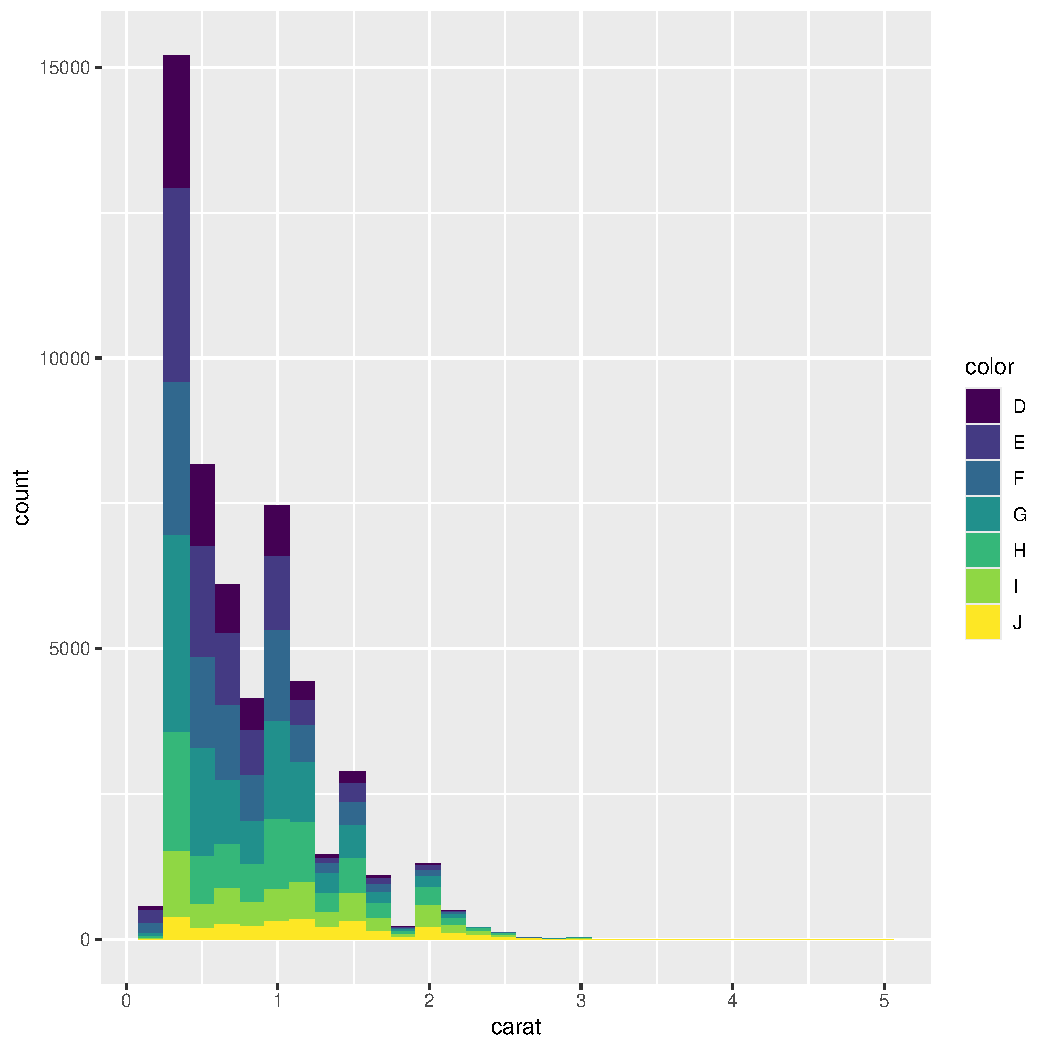
\includegraphics[width=0.75\linewidth]{C:/Users/Lewis/DataspellProjects/DataVis/Assignment/RNW/figures/Carat_and_color-1} 

}

\caption{\label{fig:fig1}plotting example}\label{fig:Carat and color}
\end{figure}

\end{knitrout}

As we can see in figure \ref{fig:fig1}

    \pagebreak
    
\begin{knitrout}
\definecolor{shadecolor}{rgb}{0.969, 0.969, 0.969}\color{fgcolor}\begin{kframe}
\begin{alltt}
\hlkwd{ggplot}\hlstd{(diamonds,} \hlkwd{aes}\hlstd{(}\hlkwc{x} \hlstd{= carat,} \hlkwc{y} \hlstd{= price))} \hlopt{+}
\hlkwd{geom_point}\hlstd{(}\hlkwd{aes}\hlstd{(}\hlkwc{color} \hlstd{= cut))}
\end{alltt}
\end{kframe}\begin{figure}[H]

{\centering 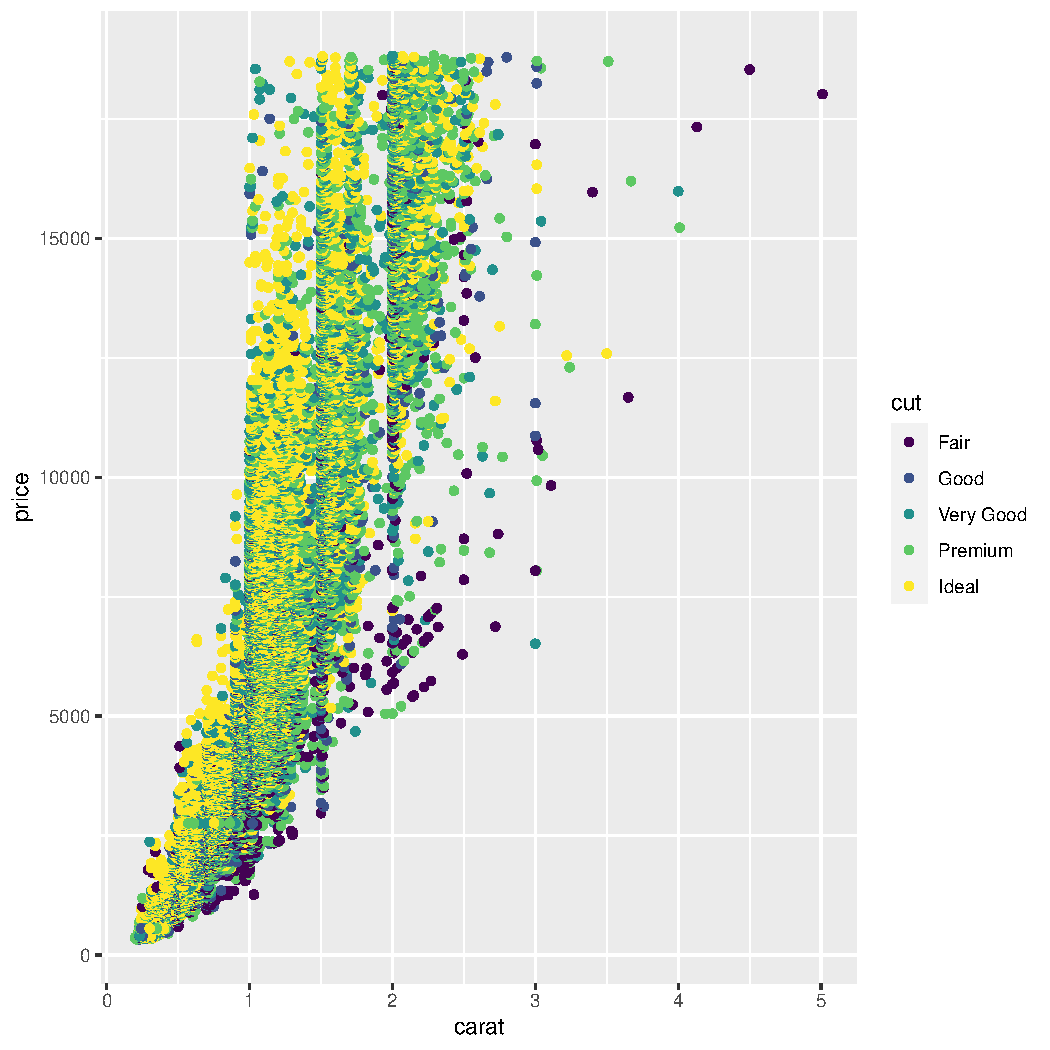
\includegraphics[width=0.75\linewidth]{C:/Users/Lewis/DataspellProjects/DataVis/Assignment/RNW/figures/Carat_and_price-1} 

}

\caption{\label{fig:fig2}plotting example 2}\label{fig:Carat and price}
\end{figure}

\end{knitrout}

Also from figure \ref{fig:fig2}

    % Declaring un-numbered chapter because I prefer how it looks.
    \chapter*{Experimental results}\label{ch:sec2}
    % Add it to the contents, because un-numbered chapters aren't by default.
    \addcontentsline{toc}{chapter}{Experimental results}
    % Put the chapter name in the header.
    \markboth{Experimental results}{}

    

\begin{knitrout}
\definecolor{shadecolor}{rgb}{0.969, 0.969, 0.969}\color{fgcolor}\begin{kframe}
\begin{alltt}
  \hlkwd{summary}\hlstd{(dataDf)}
\end{alltt}
\begin{verbatim}
##                                                 App                Category   
##  ROBLOX                                           :    9   FAMILY      :1972  
##  CBS Sports App - Scores, News, Stats & Watch Live:    8   GAME        :1144  
##  8 Ball Pool                                      :    7   TOOLS       : 843  
##  Candy Crush Saga                                 :    7   MEDICAL     : 463  
##  Duolingo: Learn Languages Free                   :    7   BUSINESS    : 460  
##  ESPN                                             :    7   PRODUCTIVITY: 424  
##  (Other)                                          :10796   (Other)     :5535  
##      Rating        Reviews                     Size             Installs   
##  Min.   : 1.0   0      : 596   Varies with device:1695   1,000,000+ :1579  
##  1st Qu.: 4.0   1      : 272   11M               : 198   10,000,000+:1252  
##  Median : 4.3   2      : 214   12M               : 196   100,000+   :1169  
##  Mean   : 4.2   3      : 175   14M               : 194   10,000+    :1054  
##  3rd Qu.: 4.5   4      : 137   13M               : 191   1,000+     : 907  
##  Max.   :19.0   5      : 108   15M               : 184   5,000,000+ : 752  
##  NA's   :1474   (Other):9339   (Other)           :8183   (Other)    :4128  
##    Type           Price               Content.Rating           Genres    
##  0   :    1   0      :10040                  :   1   Tools        : 842  
##  Free:10039   $0.99  :  148   Adults only 18+:   3   Entertainment: 623  
##  NaN :    1   $2.99  :  129   Everyone       :8714   Education    : 549  
##  Paid:  800   $1.99  :   73   Everyone 10+   : 414   Medical      : 463  
##               $4.99  :   72   Mature 17+     : 499   Business     : 460  
##               $3.99  :   63   Teen           :1208   Productivity : 424  
##               (Other):  316   Unrated        :   2   (Other)      :7480  
##          Last.Updated              Current.Ver               Android.Ver  
##  August 3, 2018: 326   Varies with device:1459   4.1 and up        :2451  
##  August 2, 2018: 304   1.0               : 809   4.0.3 and up      :1501  
##  July 31, 2018 : 294   1.1               : 264   4.0 and up        :1375  
##  August 1, 2018: 285   1.2               : 178   Varies with device:1362  
##  July 30, 2018 : 211   2.0               : 151   4.4 and up        : 980  
##  July 25, 2018 : 164   1.3               : 145   2.3 and up        : 652  
##  (Other)       :9257   (Other)           :7835   (Other)           :2520
\end{verbatim}
\begin{alltt}
\hlcom{# Replace all instances of 'NA' as a string or a blank string "" to NA.}
\hlcom{# The strings 'NA' or " " and NA are two different things to R, and only the}
\hlcom{# non-string NA is detected by functions like is.na().}
\hlstd{dataDf[(dataDf} \hlopt{==} \hlstr{'NA'} \hlopt{|} \hlstd{dataDf} \hlopt{==} \hlstr{""} \hlopt{|} \hlstd{dataDf} \hlopt{==} \hlstr{"NaN"}\hlstd{)]} \hlkwb{<-} \hlnum{NA}

\hlcom{# Output a summary of the data.}
\hlkwd{summary}\hlstd{(dataDf)}
\end{alltt}
\begin{verbatim}
##                                                 App                Category   
##  ROBLOX                                           :    9   FAMILY      :1972  
##  CBS Sports App - Scores, News, Stats & Watch Live:    8   GAME        :1144  
##  8 Ball Pool                                      :    7   TOOLS       : 843  
##  Candy Crush Saga                                 :    7   MEDICAL     : 463  
##  Duolingo: Learn Languages Free                   :    7   BUSINESS    : 460  
##  ESPN                                             :    7   PRODUCTIVITY: 424  
##  (Other)                                          :10796   (Other)     :5535  
##      Rating        Reviews                     Size             Installs   
##  Min.   : 1.0   0      : 596   Varies with device:1695   1,000,000+ :1579  
##  1st Qu.: 4.0   1      : 272   11M               : 198   10,000,000+:1252  
##  Median : 4.3   2      : 214   12M               : 196   100,000+   :1169  
##  Mean   : 4.2   3      : 175   14M               : 194   10,000+    :1054  
##  3rd Qu.: 4.5   4      : 137   13M               : 191   1,000+     : 907  
##  Max.   :19.0   5      : 108   15M               : 184   5,000,000+ : 752  
##  NA's   :1474   (Other):9339   (Other)           :8183   (Other)    :4128  
##    Type           Price               Content.Rating           Genres    
##  0   :    1   0      :10040   Everyone       :8714   Tools        : 842  
##  Free:10039   $0.99  :  148   Teen           :1208   Entertainment: 623  
##  NaN :    0   $2.99  :  129   Mature 17+     : 499   Education    : 549  
##  Paid:  800   $1.99  :   73   Everyone 10+   : 414   Medical      : 463  
##  NA's:    1   $4.99  :   72   Adults only 18+:   3   Business     : 460  
##               $3.99  :   63   (Other)        :   2   Productivity : 424  
##               (Other):  316   NA's           :   1   (Other)      :7480  
##          Last.Updated              Current.Ver               Android.Ver  
##  August 3, 2018: 326   Varies with device:1459   4.1 and up        :2451  
##  August 2, 2018: 304   1.0               : 809   4.0.3 and up      :1501  
##  July 31, 2018 : 294   1.1               : 264   4.0 and up        :1375  
##  August 1, 2018: 285   1.2               : 178   Varies with device:1362  
##  July 30, 2018 : 211   2.0               : 151   4.4 and up        : 980  
##  July 25, 2018 : 164   (Other)           :7972   (Other)           :3169  
##  (Other)       :9257   NA's              :   8   NA's              :   3
\end{verbatim}
\begin{alltt}
\hlcom{# Identify rows containing NA.}
\hlstd{naRows} \hlkwb{<-} \hlstd{dataDf[}\hlkwd{rowSums}\hlstd{(}\hlkwd{is.na}\hlstd{(dataDf))} \hlopt{>} \hlnum{0}\hlstd{,]}
\hlcom{# 1469 with no ratings, 8 with no current version, 4 with neither}
\hlkwd{nrow}\hlstd{(naRows)}
\end{alltt}
\begin{verbatim}
## [1] 1481
\end{verbatim}
\end{kframe}
\end{knitrout}

    % Declaring un-numbered chapter because I prefer how it looks.
    \chapter*{Summary \& conclusion}\label{ch:sec3}
    % Add it to the contents, because un-numbered chapters aren't by default.
    \addcontentsline{toc}{chapter}{Summary and conclusion}
    % Put the chapter name in the header.
    \markboth{Summary and conclusion}{}

    aaa

\end{document}
